\documentclass[11pt]{article}
\usepackage[utf8]{inputenc}
\usepackage[T1]{fontenc}
\usepackage{minted}
\usepackage{multirow}
\usepackage{enumerate}
\usepackage{tikz}

%% for listings..
\newminted{perl}{linenos, bgcolor=mintedBg, fontsize=\footnotesize}
\newminted{r}{linenos, bgcolor=mintedBg, fontsize=\footnotesize}
\definecolor{mintedBg}{rgb}{0.95, 0.95, 0.95}
\definecolor{blockBg}{rgb}{0.6, 0.6, 0.95}

\begin{document}

\section{Instructions}
This (example) exam contains questions with marks totalling up to 167 points.
100 points will give full marks. You are free to choose any set of questions, but
marks will only be awarded for the first set of questions that total up to 100.
If you have started an answer, and find that you are not satisifed with it, you can
cross it out and replace it with an answer to a later question.

Marks have been assigned on the assumption of a four hour exam; that is one mark
corresponds to 2.4 minutes. For some of the questions that may mean mostly
writing, but for others (esp. code snippets) that time may be taken up by
reading the details of the question, and the answer itself may be very short.

If the marks available for your answers do not add up to exactly 100 marks, then the
marks awarded to the last question answered (i.e. the one whose marks bring the total
score available to more than 100 points) will be awarded fully, potentially allowing
you to exceed a perfect score.

\section{Bioinformatics in General}
\begin{enumerate}
\item Describe some examples of problems and fields addressed by
  Bioinformatics. Full marks require at least three examples; points
  will be given both for depth of explanation and for numbers of points.\\
  (4 points)
\item Why is an understanding of bioinformatics becoming essential for
  the study of biology? Give some examples to illustrate your answer.\\
  (3 points)
\item Why is there such an emphasis of the analysis of sequences within
  bioinformatics? (Any reasonable answer will be accepted).\\
  (2 points)
\item Describe and contrast how genes were identified before and after the
  availability of cheap DNA sequencing.\\
  (4 points)
\end{enumerate}

\section{Molecular Biology \& the Central Dogma}  
\begin{enumerate}
\item Describe the structure of genes in both prokaryotes and
  eukaryotes.Include as many features as you can.
  \begin{itemize}
  \item How do we usually define a gene? How does this differ
    from the historical definition of a gene.
  \item Discuss what should be included as part of a gene
    and how this makes it difficult to define the number of genes an organism
    has.
  \end{itemize}
  (10 points)
\item Describe the central dogma, including exceptions to the general rule.\\
  (7 points)
\item What do we mean when we say that two nucleic acid sequences (DNA or RNA) are
  complementary?\\
  (2 points)
\item The majority of DNA molecules are double stranded, whereas the majority of
  RNA molecules are single stranded. Discuss the role of strandedness in the
  function of DNA.\\
  (3 points)
\item How do the monomers of nucleic acids differ from those of proteins? How
  does this relate to their function?\\
(4 points)
\item What are exons and introns?\\
(3 points)
\item What is a codon? How long is it and why?\\
(4 points)
\item What do we mean when we talk about the degeneracy of the genetic code?\\
(2 points)
\item Given a genetic code:\\
  \begin{minipage}{0.6\textwidth}
  {\tiny
    %% this requires 
%% usepackage{multirow}
%% usepackage{tabularx}

\renewcommand{\arraystretch}{1.25}
\begin{tabular}{ |l| l l|l l| l l|l l|l| }
  \hline
  \multirow{2}{2em}{1st base} &
  \multicolumn{8}{|c|}{2nd base} &
  \multirow{2}{2em}{3rd base} \\
  \cline{2-9}
  &
  \multicolumn{2}{|c|}{U} &
  \multicolumn{2}{|c|}{C} &
  \multicolumn{2}{|c|}{A} &
  \multicolumn{2}{|c|}{G} & \\
  \hline
  \multirow{4}{2em}{U} & 
  UUU & \multirow{2}{4em}{\tiny (Phe/F)} &
  UCU & \multirow{4}{4em}{\tiny (Ser/S)} &
  UAU & \multirow{2}{4em}{\tiny (Tyr/Y)} &
  UGU & \multirow{2}{4em}{\tiny (Cys/C)} & U \\
  & UUC & & UCC & & UAC & & UGC & & C \\ \cline{2-3} \cline{6-9}
  & UUA & \multirow{6}{4em}{\tiny (Leu/L)} 
  & UCA & & UUA & Stop & UGA & (Stop) & A \\ \cline{8-9}
  & UUG & & UCG & & UAG & Stop & UGG & \tiny (Trp/W) & G \\ \cline{4-9} 
  \cline{1-1}
  \multirow{4}{2em}{C}
  & CUU & & CCU & \multirow{4}{4em}{(Pro/P)} & CAU & \multirow{2}{4em}{(His/H)} & CGU & \multirow{4}{4em}{(Arg/R)} & U \\
  & CUC & & CCC & & CAC & & CGC & & C \\ \cline{6-7}
  & CUA & & CCA & & CAA & \multirow{2}{4em}{Gln/Q} & CGA & & A \\
  & CUG & & CCG & & CAG & & CGG & & G \\ \cline{1-9}
  \multirow{4}{2em}{A}
  & AUU & \multirow{3}{4em}{(Ile/I)} & ACU & \multirow{4}{4em}{(Thr/T)} & AAU 
  & \multirow{2}{4em}{(Asn/N)} & AGU & \multirow{2}{4em}{(Ser/S)} & U \\
  & AUC & & ACC & & AAC & & AGC & & C \\ \cline{6-9}
  & AUA & & ACA & & AAA & \multirow{2}{4em}{(Lys/K)} & AGA & \multirow{2}{4em}{(Arg/R)} & A \\
  \cline{2-3}
  & AUG & (Met/M) & ACG & & AAG & & AGG & & G \\ \cline{1-9}
  \multirow{4}{4em}{G}
  & GUU & \multirow{4}{4em}{(Val/V)} & GCU & \multirow{4}{4em}{(Ala/A)} 
  & GAU & \multirow{2}{4em}{(Asp/D)} & GGU & \multirow{4}{4em}{(Gly/G)} & U \\
  & GUC & & GCC & & GAC & & GGC & & C \\ \cline{6-7}
  & GUA & & GCA & & GAA & \multirow{2}{4em}{(Glu/E)} & GGA & & A \\
  & GUG & & GCG & & GAG & & GGG & & G \\ \hline
\end{tabular}

  }
  \end{minipage}

  Give all the amino acide sequences that can be encoded by:\\
  \verb|ATGAGATAAGATATCTACG|\\
  (4 points)
\item What kind of mutations can arise in DNA sequences? What effects
  do the different types of mutations have on genes?\\
  (4 points)
\end{enumerate}  

\section{Biological databases}
\begin{enumerate}
\item Describe examples of the types of data that is held in different
  databases. Comment on how the type of data affects how the data is stored
  and accessed.\\
  (3 points)
\item Where can you find DNA sequences? (If you have trouble remembering
  specific names of databases, describe in some detail how you would go about finding a
  location / database that gives you DNA sequences).\\
  (3 points)
\item Given a database of sequences how can you obtain relevant sequences? Note
  that this depends both on your starting point (i.e. the information that
  you begin with) and what you want to do with the sequences. Describe at least two
  different scenarios.
  (5 points)
\item How would you find biological information about a given DNA sequence?
  Include details about the type of information that can be encoded by a DNA
  sequence and how this relates to your choice of database.
  (remember the structure of genes).\\
  (3 points)
\item Apart from sequence data what does the fastq format contain?\\
  (1 point)
\item What are genome databases and why are they useful?\\
  (4 points)
\item Describe the fasta format.\\
  (2 points)
\end{enumerate}

\section{Pairwise alignment}
\begin{enumerate}
\item For the two sequences: \verb|5' GCATGGTA 3'| and \verb|5' TCCATG 3'| :
  \begin{enumerate}
    \item Provide three reasonable alignments (feel free to change strandedness).
    \item Describe how you can score the alignments using sets of penalties
      (remember that you can have negative penalties).
    \item Score the alignments using at least two different sets of
      penalties. Comment on how the choice of penalties relates to the
      biological question being asked.
    \item Which of your alignments do you think is most reasonable and why? If you
      think all are equally reasonable then explain your opinion.
  \end{enumerate}
  (10 points)
\item Why do we often use a different penalty for gap insertion and gap
  extension? Provide an example alignment with your question.\\
  (4 points)
\item What do we mean by an optimal alignment?\\
  (2 points)
\item Fill in the first three rows and columns of the following
  alignment table for a local alignment (Smith-Waterman). Include
  both scores and back-track information.
  \begin{figure}[H]
    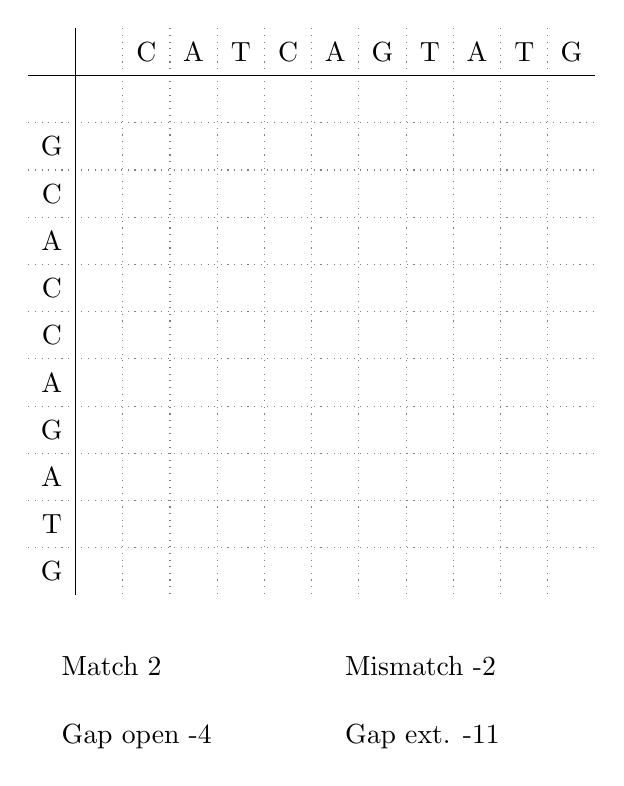
\begin{tikzpicture}[scale=0.6]
      \node [right] at (1,-1) {Match 2};
\node [right] at (7,-1) {Mismatch -2};
\node [right] at (1,-2.5) {Gap open -4};
\node [right] at (7,-2.5) {Gap ext. -11};

\draw [-] (0.5,11.5) -- (12.5,11.5);
\draw [-] (1.5,12.5) -- (1.5,0.5);
\draw [-, dotted, opacity=0.5] (0.5,10.5) -- (12.5,10.5);
\draw [-, dotted, opacity=0.5] (2.5,12.5) -- (2.5,0.5);
	\node at (3,12) {C};
	\draw [-, dotted, opacity=0.5] (3.5,12.5) -- (3.5,0.5);
	\node at (4,12) {A};
	\draw [-, dotted, opacity=0.5] (4.5,12.5) -- (4.5,0.5);
	\node at (5,12) {T};
	\draw [-, dotted, opacity=0.5] (5.5,12.5) -- (5.5,0.5);
	\node at (6,12) {C};
	\draw [-, dotted, opacity=0.5] (6.5,12.5) -- (6.5,0.5);
	\node at (7,12) {A};
	\draw [-, dotted, opacity=0.5] (7.5,12.5) -- (7.5,0.5);
	\node at (8,12) {G};
	\draw [-, dotted, opacity=0.5] (8.5,12.5) -- (8.5,0.5);
	\node at (9,12) {T};
	\draw [-, dotted, opacity=0.5] (9.5,12.5) -- (9.5,0.5);
	\node at (10,12) {A};
	\draw [-, dotted, opacity=0.5] (10.5,12.5) -- (10.5,0.5);
	\node at (11,12) {T};
	\draw [-, dotted, opacity=0.5] (11.5,12.5) -- (11.5,0.5);
	\node at (12,12) {G};
	\node at (1,10) {G};
	\draw [-, dotted, opacity=0.5] (0.5,9.5) -- (12.5,9.5);
	\node at (1,9) {C};
	\draw [-, dotted, opacity=0.5] (0.5,8.5) -- (12.5,8.5);
	\node at (1,8) {A};
	\draw [-, dotted, opacity=0.5] (0.5,7.5) -- (12.5,7.5);
	\node at (1,7) {C};
	\draw [-, dotted, opacity=0.5] (0.5,6.5) -- (12.5,6.5);
	\node at (1,6) {C};
	\draw [-, dotted, opacity=0.5] (0.5,5.5) -- (12.5,5.5);
	\node at (1,5) {A};
	\draw [-, dotted, opacity=0.5] (0.5,4.5) -- (12.5,4.5);
	\node at (1,4) {G};
	\draw [-, dotted, opacity=0.5] (0.5,3.5) -- (12.5,3.5);
	\node at (1,3) {A};
	\draw [-, dotted, opacity=0.5] (0.5,2.5) -- (12.5,2.5);
	\node at (1,2) {T};
	\draw [-, dotted, opacity=0.5] (0.5,1.5) -- (12.5,1.5);
	\node at (1,1) {G};



    \end{tikzpicture}
  \end{figure}
  (3 points)
\item What does the following figure contain?
  Obtain all optimal alignments from it:
  \begin{figure}[H]
    \begin{tikzpicture}[scale=0.6]
      \input{nm2_aa.tikz}
    \end{tikzpicture}
  \end{figure}
  \begin{enumerate}
  \item Draw the process directly on the table.
  \item What kind of alignment(s) did you obtain?
  \end{enumerate}
  (4 points)
\item The following is an example of an amino acid substitution table.
  \begin{figure}[H]
    \includegraphics[width=0.9\textwidth]{images/dayhoff_256}
  \end{figure}
  \begin{enumerate}
  \item The table has high and low values. What do these mean?
  \item What do the numbers along the diagonal indicate? Why do they
    vary?
  \end{enumerate}
  (4 points)
\item Describe at least two ways in which you can derive an amino acid
  substitution matrix?\\
  (4 points)
\end{enumerate}

\section{Multiple sequence alignment}
\begin{enumerate}
\item What are homologues, orthologues and paralogues?\\
  (4 points)
\item Describe some uses of multiple sequence alignment.\\
  (3 points)
\item How does Clustal create alignments from multiple
  sequences?\\
  (5 points)
\item Why do we not use dynamic programming for multiple
  sequence alignment? What kind of methods do we use
  instead?\\
  (2 points)
\end{enumerate}

\section{Perl}
\begin{enumerate}
\item What is Perl, and what is it useful for?\\
  (2 points)
\item What are the three ways in which you can store values in Perl? Give
  examples as to how you can assign values to such variables?\\
  (4 points)
\item What does the following code do?

  \begin{perlcode}
  #!/usr/bin/perl -w
    
  $a = $ARGV[0];
  $b = $ARGV[1];

  print "$a + $b = ", $a + $b, "\n";
  \end{perlcode}
  Explain what kind of errors you may get running the above code.\\
  (4 points)
\item 
  The Fibonacci sequence is defined as a sequence of numbers starting
  with 1,1 or 0,1 and where every subsequent number is the sum of the two
  previous numbers. That is: $F_i = F_{i-2} + F_{i-1}$. Write a small piece
  of Perl that calculates and prints the first 100 values of the Fibonacci
  sequence. (You will be minimally penalised for syntax errors, the logic is
  more important).\\
  (5 points)
\item What is the difference between:

  \begin{perlcode}
  if($a eq $b)
  \end{perlcode}
  and

  \begin{perlcode}
  if($a == $b)
  \end{perlcode}
  When would you use one rather than the other?\\
  (2 points)
\item What will the following code print:

  \begin{perlcode}
  $a = 10;
  $b = 8;
  if($a = $b){
    print "$a is equal to $b\n";
  }else{
    print "$a is not equal to $b\n";
  }
  \end{perlcode}
  Read carefullly...\\
  (2 points)
\end{enumerate}

\section{Searching databases by sequence}
\begin{enumerate}
\item Describe the relationship between pairwise sequence alignment and
  searching a database of sequences for homologous sequences.\\
  (3 points)
\item When would you use Blat as opposed to Blast?\\
  (2 points)
\item Write down a lookup table (index) for the following sequence:
\begin{verbatim}
TPATGGANWT
\end{verbatim}
 (3 points)
\item Why do we not normally use a dynamic programming method to identify
  homologous sequences.\\
  (1 point)
\item You have searched a database for homologous sequences and have obtained
  the following results:
\begin{figure}[H]
  \input{database_alignments_2.tikz}
\end{figure}
{\small(db 1, db 2, etc..., refer to individual sequences within the database, the
thickness of the diagonal lines refer to local alignment scores)}\\
What can you infer from these alignments? How does the choice of database
affect the inferences that you can make?\\
(4 points)
\item How would you identify a local alignment between sequence 1 (\verb|LGALSCTCW|) 
  and 2 (\verb|GSLLCTA|) from the following table:
\begin{figure}[H]
  \begin{minipage}[t]{0.5\textwidth}
  {\small
    \setlength{\tabcolsep}{0.5em}
    \begin{tabular}[t]{l|ll|l}
      AA & S2 & S1 & S1-S2 \\
      \hline
      G & 1 & 2 & 1\\
      S & 2 & 5 & 3\\
      L & 3 & 1,4 & -2,1 \\
      L & 4 & 1,4 & -3,0\\
      C & 5 & 6 & 1\\
      T & 6 & 7 & 1\\
      A & 7 & 3 & -4 \\
    \end{tabular}
  }
\end{minipage} 
\begin{minipage}[t]{0.5\textwidth}
  {\small
  Where, \texttt{AA} gives the amino acid residues in sequence 2 located at
  the positions indicated by column \texttt{S2}. Column \texttt{S1} gives
  the lookup table for sequence one. Column \texttt{S1-S2} gives the
  difference between values in \texttt{S1} and \texttt{s2}.
  }
\end{minipage}
  

\end{figure}
Write out the final alignment and score it using the substitution matrix
given in the pairwise alignment section.
{\small Hints: It may help you to plot column \texttt{S1} vs
  \texttt{S2}, though this is not necessary.
}\\
(6 points)
\item The following image shows the graphical output from an NCBI blast
  search. What can you tell from the picture?
  \begin{figure}[H]
    \includegraphics[width=0.9\textwidth]{images/blast_result_image}
  \end{figure}
  (3 points)
\end{enumerate}

\section{Numbers, big data and R}
\begin{enumerate}
\item Describe the three most commonly used average values.\\
  (3 points)
\item What is meant by 'the distribution of values' and how can you obtain
  this in \texttt{R}?\\
  (3 points)
\item What is meant by, a) a normal distribution and b) a log normal
  distribution? Sketch suitable plots to illustrate your explanation.\\
  (3 points)
\item Describe how you can obtain p-value from an arbitrary statistic (eg.
  the t-statistic).\\
  (4 points)
\item The following R-code creates some matrices:

  \begin{rcode}
    a <- matrix(1:9, ncol=3, byrow=TRUE)
    b <- t(a)
    c <- rbind(a, b)
    d <- c[ rowSums(c) > 10, 2:3]
    e <- a + b[1,]
  \end{rcode}
  Draw the resulting matrices.\\
  (4 points)
\item What will the following code do:

  \begin{rcode}
    phrases <- c("hello there stranger", "what's up doc")
    words <- strsplit(phrases, " ")
    words <- unlist(words)
    sort(words)
  \end{rcode}
  Describe what each line of code does and the output of the
  final line of code.\\
  (4 points)
\item Given a big data set (e.g. expression values for all
  known genes over a series of conditions) give an outline of
  how you can determine the relationships between samples
  and identify genes with interesting expression patterns.\\
  (10 points)
\item Describe the types of data you should include in big data set
  analyses (consider the experimental design, implementation and
  the final data)?\\
  (6 points)
\end{enumerate}

\section{Databases}
\begin{enumerate}
\item What is a database? Describe how data is organised in; flat file,
  relational and object orientated databases. Give examples for types
  of data that may be suitable for the different database types.\\
  (5 points)
\item Describe a relational structure (i.e. a set of tables) that would be
  suitable for storing information about genes (e.g. gene locations, names,
  associated transcripts and exons). Use a simple sketch to illustrate the
  tables, columns and their relationships of your design. (If the meaning of
  your drawing is not completely clear you may wish to add an explanatory
  figure label).\\
  (6 points)
\end{enumerate}

\end{document}